%!TEX root = /Users/fgeerts/Documents/MLforloops/pods/main.tex
The real work begins here.

\section{ARA}
\newcommand{\MLm}{\mathsf{MATLANG}}
\newcommand{\ML}{$\MLm$\xspace}
\newcommand{\ARAm}{\mathsf{ARA}}
\newcommand{\ARA}{$\ARAm$\xspace}
\newcommand{\ARAC}{$(\ARAm+\zeta_k)(k)$\xspace}
\newcommand{\ARACTWO}{$(\ARAm+\zeta_2)(2)$\xspace}
\newcommand{\Rel}{\mathrm{Rel}}
\newcommand{\Mat}{\mathrm{Mat}}

% \DeclareMathOperator{\sdiff}{\triangle}
% By \emph{function} we will always mean a total function. For a function $f: X \to Y$ and $Z \subseteq X$, the \emph{restriction} of $f$ to $Z$, denoted by $f|_Z$, is the function $Z \to Y$ where $f|_Z(x) = f(x)$ for all $x \in Z$.

%
%
%
% From the outset, we also fix countable infinite sets $\mathbf{rel}$, $\mathbf{att}$, and $\mathbf{dom}$, the elements of which are called \emph{relation names}, \emph{attributes}, and \emph{domain elements}, respectively. We assume an equivalence relation $\sim$ on $\mathbf{att}$ that partitions $\mathbf{att}$ into an infinite number of equivalence classes that are each infinite. When $A \sim B$, we say that $A$ and $B$ are \emph{compatible}. Intuitively, $A \sim B$ will mean that $A$ and $B$ have the same set of domain values. A function $f: X \to Y$ with $X$ and $Y$ sets of attributes is called \emph{compatible} if $f(A) \sim A$ for all $A \in X$.
%
\subsection{Annotated-Relation Algebra (\ARA)} 
For completeness, we start by recalling the definition of the \ARA query language. We  here closely follow the exposition given in~\cite{brijder2019matrices}.

Let $\mathbf{att}$ and $\mathbf{dom}$ denote countable infinite sets of  \emph{attributes} and \emph{domain elements}, respectively. A notion of compatibility between attributes is assumed. More formally,
we assume that an equivalence relation $\sim$ on $\mathbf{att}$ is present which partitions $\mathbf{att}$ into an infinite number of equivalence classes that are each infinite. When $A \sim B$, we say that $A$ and $B$ are \emph{compatible}. Intuitively, $A \sim B$ will mean that $A$ and $B$ have the same set of domain values. A function $f: X \to Y$ with $X$ and $Y$ sets of attributes is called \emph{compatible} if $f(A) \sim A$ for all $A \in X$.

A \emph{relation schema} is a finite subset of $\mathbf{att}$. A \emph{database schema} is a function $\mathcal{R}$ on a finite set $N$ of relation names, assigning a relation schema $\mathcal{R}(R)$ to each $R \in N$.
% The \emph{arity} of a relation name $R$ is the cardinality $|\mathcal{R}(R)|$ of its schema. The \emph{arity} of $\mathcal{R}$ is the largest arity among relation names $R \in N$.

The \emph{(positive) Annotated-Relation Algebra}, abbreviated by \ARA, is defined as follows. With each expression $\varphi$ in \ARA one also assigns a relation schema $\mathcal{R}(\varphi)$, by extending the initial schema
$\mathcal{R}$. An \emph{\ARA expression} $\varphi$ over a database schema $\mathcal{R}$ is equal to 
\begin{itemize}
\item a relation name $R$ of $\mathcal{R}$;
\item $\mathbf{1}(\psi)$, where $\psi$ is an \ARA expression, and $\mathcal{R}(\varphi) := \mathcal{R}(\psi)$;
\item $\psi_1 \cup \psi_2$, where $\psi_1$ and $\psi_2$ are \ARA expressions with $\mathcal{R}(\psi_1) = \mathcal{R}(\psi_2)$, and $\mathcal{R}(\varphi) := \mathcal{R}(\psi_1)$;
\item $\pi_Y(\psi)$, where $\psi$ is an \ARA expression and $Y \subseteq \mathcal{R}(\psi)$, and $\mathcal{R}(\varphi) := Y$;
% \item $\pi_Y^\star(\psi)$, where $\psi$ is an \ARA expression and $Y \subseteq \mathcal{S}(\psi)$, and $\mathcal{S}(\varphi) := Y$;
\item $\sigma_{Y}(\psi)$, where $\psi$ is an \ARA expression, $Y \subseteq \mathcal{R}(\psi)$, the elements of $Y$ are mutually compatible, and $\mathcal{R}(\varphi) := \mathcal{R}(\psi)$;
\item $\rho_{\mathcal{R}(\psi) \mapsto Y}(\psi)$, where $\psi$ is an \ARA expression and $\mathcal{R}(\psi) \mapsto Y$ is a compatible one-to-one correspondence of attributes with $Y \subseteq \mathbf{att}$, and $\mathcal{R}(\varphi) := Y$; or
\item $\psi_1 \Join \psi_2$, where $\psi_1$ and $\psi_2$ are \ARA expressions, and $\mathcal{R}(\varphi) := \mathcal{R}(\psi_1) \cup \mathcal{R}(\psi_2)$.
\end{itemize}

We next define the semantics of \ARA expression.
A \emph{domain assignment} is a function $\mathbb{D}: \mathbf{att} \to
2^{\mathbf{dom}}$ such that $A \sim B$ implies
$\mathbb{D}(A) = \mathbb{D}(B)$. Let $X$ be a relation schema. A \emph{tuple} over
$X$ with respect to $\mathbb{D}$
is a function $t: X \to \mathbf{dom}$ such that
$t(A) \in \mathbb{D}(A)$ for all $A \in X$. We denote by
$\mathcal{T}_{\mathbb{D}}(X)$ the set of tuples over $X$ with respect to $\mathbb{D}$. Note that
$\mathcal{T}_{\mathbb{D}}(X)$ is finite.  A \emph{relation} $r$ over
$X$ with respect to $\mathbb{D}$ is a function $r:
\mathcal{T}_{\mathbb{D}}(X) \to K$ for a \emph{semiring} $(K,+,*,0,1)$. So a relation annotates every tuple
over $X$ with respect to $\mathbb{D}$ with a value from $K$.  If $\mathcal{R}$ is a
database schema, then an \emph{instance $\mathcal{I}$ of
$\mathcal{R}$ with respect to $\mathbb{D}$} is a function that assigns to every
relation name $R$ of $\mathcal{R}$ a relation $\mathcal{I}(R):
\mathcal{T}_{\mathbb{D}}(\mathcal{R}(R)) \to K$.

The semantics of \ARA expressions is defined, as follows.

\begin{description}


\item[One] For every relation schema $X$,
  we define $\mathbf{1}_X: \mathcal{T}_{\mathbb{D}}(X) \to K$ where $\mathbf{1}_X(t) = 1$ for every $t \in \mathcal{T}_{\mathbb{D}}(X)$. 


\item[Union] Let $r_1, r_2: \mathcal{T}_{\mathbb{D}}(X) \to K$. Define $r_1 \cup r_2: \mathcal{T}_{\mathbb{D}}(X) \to K$ as $(r_1 \cup r_2)(t) = r_1(t) + r_2(t)$.


\item[Projection] Let $r: \mathcal{T}_{\mathbb{D}}(X) \to K$ and $Y \subseteq X$. Define $\pi_{Y}(r): \mathcal{T}_{\mathbb{D}}(Y) \to K$ as
\[
(\pi_{Y}(r))(t) = \sum_{\substack{t' \in \mathcal{T}_{\mathbb{D}}(X),\\ t'|_{Y} = t}} \!\! r(t').
\]


\item[Selection] Let $r: \mathcal{T}_{\mathbb{D}}(X) \to K$ and $Y \subseteq X$ where the elements of $Y$ are mutually compatible. Define $\sigma_{Y}(r): \mathcal{T}_{\mathbb{D}}(X) \to K$ such that
\[
(\sigma_{Y}(r))(t) =
\begin{cases}
r(t) & \text{if } t(A)=t(B) \text{ for all } A, B \in Y;\cr
0    & \text{otherwise}.
\end{cases}
\]


\item[Renaming] Let $r: \mathcal{T}_{\mathbb{D}}(X) \to K$ and $\varphi: X \to Y$ a compatible one-to-one correspondence. We define $\rho_\varphi(r): \mathcal{T}_{\mathbb{D}}(Y) \to K$ as $\rho_\varphi(r)(t) = r(t \circ \varphi)$.

\item[Join] Let $r_1: \mathcal{T}_{\mathbb{D}}(X_1) \to K$ and $r_2: \mathcal{T}_{\mathbb{D}}(X_2) \to K$. Define $r_1 \Join r_2: \mathcal{T}_{\mathbb{D}}(X_1 \cup X_2) \to K$ as $(r_1 \Join r_2)(t) = r_1(t|_{X_1})*r_2(t|_{X_2})$.
\end{description}

The above operations provide semantics for \ARA in a natural manner. Formally, let $\mathcal{R}$ be a database schema, let $\varphi$ be an \ARA expression over $\mathcal{R}$, and let $\mathcal{I}$ be an instance of $\mathcal{R}$. The \emph{output} relation $\varphi(\mathcal{I})$ of $\varphi$ under $\mathcal{I}$ is defined as follows. If $\varphi = R$ with $R$ a relation name of $\mathcal{R}$, then $\varphi(\mathcal{I}) := \mathcal{I}(R)$. If $\varphi = \mathbf{1}(\psi)$, then $\varphi(\mathcal{I}) := \mathbf{1}_{\mathcal{S}(\psi)}$. If $\varphi = \psi_1 \cup \psi_2$, then $\varphi(\mathcal{I}) := \psi_1(\mathcal{I}) \cup \psi_2(\mathcal{I})$. If $\varphi = \pi_{X}(\psi)$, then $\varphi(\mathcal{I}) := \pi_{X}(\psi(\mathcal{I}))$. If $\varphi = \sigma_{Y}(\psi)$, then $\varphi(\mathcal{I}) := \sigma_{Y}(\psi(\mathcal{I}))$. If $\varphi = \rho_\varphi(\psi)$, then $\varphi(\mathcal{I}) := \rho_\varphi(\psi(\mathcal{I}))$. Finally, if $\varphi = \psi_1 \Join \psi_2$, then $\varphi(\mathcal{I}) := \psi_1(\mathcal{I}) \Join \psi_2(\mathcal{I})$.


\subsection{An extension of \ARA}
We extend \ARA with the following two operators:
\begin{itemize}
 \item $\pi_Y^\star(\psi)$, where $\psi$ is an \ARA expression and $Y \subseteq \mathcal{R}(\psi)$, and $\mathcal{R}(\varphi) := Y$;
 \item $\textsf{Apply}[f](\psi_1,\ldots,\psi_k)$, where $\psi_1,\ldots,\psi_k$ are \ARA expressions with $\mathcal{R}(\psi_1)=\cdots=\mathcal{R}(\psi_k)$, 
 $f$ is a function $K^k\to K$,
 and 
 $\mathcal{R}(\varphi)=\mathcal{R}(\psi_1)$.
\end{itemize}
The semantics of these operators is given by:
\begin{description}
\item[$\star$-Projection] Let $r: \mathcal{T}_{\mathbb{D}}(X) \to K$ and $Y \subseteq X$. Define $\pi_{Y}^\star(r): \mathcal{T}_{\mathbb{D}}(Y) \to K$ as
\[
(\pi_{Y}(r))(t) = \prod_{\substack{t' \in \mathcal{T}_{\mathbb{D}}(X),\\ t'|_{Y} = t}} \!\! r(t').
\]
\item[Function application] Let $r_{i}: \mathcal{T}_{\mathbb{D}}(X) \to K$ for $i=1,\ldots,k$. Define $\textsf{Apply}[f](r_1,\ldots,r_k): \mathcal{T}_{\mathbb{D}}(Y) \to K$ as
\[
(\textsf{Apply}[f](r_1,\ldots,r_k))(t) = f(r_1(t),\ldots,r_k(t)).
\]
\end{description}
Hence, if $\varphi=\pi^\star_{Y}(\psi)$ then 
$\varphi(\mathcal{I}):=\pi^\star_{Y}(\psi(\mathcal{I}))$, and
if $\varphi=\textsf{Apply}[f](\psi_1,\allowbreak \ldots,\psi_k)$ then we have
$\varphi(\mathcal{I}):=\textsf{Apply}[f](\psi_1(\mathcal{I}), \ldots,\psi_k(\mathcal{I}))$. We let $\Omega$ denote a set of pointwise functions that can be used in function applications and write \ARA$_\Omega$ to make this explicit.


\subsection{Upper bound on expressivity}
There is a straightforward translation from \ARA$_{\Omega}$ expressions into the relational algebra with aggregation $\text{ALG}_{\text{aggr}}(\Omega',\Theta)$ as defined in~\cite{LIBKIN2003}. Here, $\Omega'$ consists of the functions in $\Omega$ and complemented with the unary functions $1:K\to K:k\mapsto 1$, to deal with $\mathbf{1}$ operator and $0:K\to K:k\mapsto 0$ to deal with selection and binary functions $f_+:K^2\to K:(k,\ell)\mapsto k+\ell$ and $f_*:K^2\to K:(k,\ell)\mapsto k*\ell$.
Furthermore, $\Theta$ consist of aggregate functions corresponding to the semiring sum and product, lifted to multi-sets. More precisely,
$\Theta$ includes $f_+^1,f_+^2,f_+^3,\ldots$ such that $f_+^n$ maps
$n$-element multi-sets in $K$ to their sum, and 
 $f_*^1,f_*^2,f_*^3,\ldots$ such that $f_*^n$ maps
 $n$-element multi-sets in $K$ to their product.

The language $\text{ALG}_{\text{aggr}}(\Omega,\Theta)$ is defined over a ``pure'' relational schema in which attributes are typed. It is easy to see that with every \ARA schema $\mathcal{R}$ we can associate a relational schema encoding the same information. Intuitively, we have one attribute of type $\mathbf{dom}$ for each $A\in\mathcal{R}$ and a special attribute $\text{Val}$ of type $K$ which is to hold the semiring values.

Given this translation, it is known that every expression in  $\text{ALG}_{\text{aggr}}(\Omega,\Theta)$ corresponds to an expression in the finite rank fragment $\mathcal{L}_{\infty,\omega}^*(\textbf{Cnt})$ of infinitary logic with counting $\mathcal{L}_{\infty,\omega}(\textbf{Cnt})$~\cite{LIBKIN2003,Hella:2001}. 
Since this logic is local, \ARA inherits this locality. As an example, 
transitive closure and connectivity of graphcs cannot be expressed in \ARA$_{\Omega}$.

\section{\lang$(\sum,\prod)$}
\newcommand{\row}{\mathsf{row}}
\newcommand{\rows}{\mathsf{rows}}
\newcommand{\col}{\mathsf{col}}
\newcommand{\cols}{\mathsf{cols}}

We next show that \lang$(\Sigma)$ and \ARA are closely connected. To make this correspond formal we first establish a link between matrix schemas and relation schemas, and matrix instances and database instances.

We start from a matrix schema $\Sch=(\Mnam,\size)$, where $\Mnam\subset \Mvar$ is a finite set of matrix variables, and $\size: \Mvar \mapsto \DD\times \DD$ is a function that maps each matrix variable to a pair of size symbols. On the relational side
we have for each size symbol $\alpha\in\DD\setminus\{1\}$, attributes $\row_\alpha$ and $\col_\alpha$ in $\mathbf{att}$. Given
$\Sch$, the domain asssignment $\mathbb{D}_\Sch$ is defined as 
$\mathbb{D}_\Sch(\row_\alpha)=[1,\size(\alpha)]$ and 
$\mathbb{D}_\Sch(\col_\alpha)=[1,\size(\alpha)]$. We define the database  schema $\text{Rel}(\Sch)$ such that for each $V\in\Mnam$,
\[
	\text{Rel}(\Sch)(V) = \begin{cases}
		\lbrace\row_\alpha,\col_\beta \rbrace & \text{ if $ \size(V)=(\alpha,\beta)$} \\
		\lbrace\row_\alpha \rbrace & \text{ if $ \size(V)=(\alpha,1)$} \\
		\lbrace\col_\beta \rbrace  &
	 \text{ if $ \size(V)=(1,\beta)$} \\
		\lbrace\rbrace & \text{ if $\size(V)=(1,1)$}.
\end{cases}
\]
Consider a matrix instance $\I = (\dom,\conc)$ over a schema $\Sch$.
Let $V\in\Mnam$ with $\size(V)=(\alpha,\beta)$ and $\conc(V)$ be its corresponding matrix of dimension $\dom(\alpha)\times \dom(\beta)$.
We then define the database instance $\text{Rel}_\Sch(\I)$  to consist of relations for each $V\in\Mnam$ defined as follows:
$\mathcal{T}_{\mathbb{D}_{\Sch}}(\text{Rel}(\Sch)(V)) \to K$ such that
$(\text{Rel}_{_\Sch}(I))(t):=\conc(V)_{ij}$ where (1) $t(\row_\alpha)=i$ if $\alpha\neq 1$ and equal to $1$ if $\alpha = 1$; and (2) $t(\col_\beta)=j$ if $\beta\neq 1$ and equal to $1$ if $\beta= 1$.

We next translate \lang++ expressions $e$ into \ARA expressions $\Phi(e)$ by induction on the structure.
%
% \begin{itemize}
% 	\item If $e=V$ then $\Phi(e):=\text{Rel}(\Sch)(V)$.
% 	\item if $e=e^t$ then \[
% \Phi(e) :=
% \begin{cases}
% \rho_{\varphi}(\Phi(e')) & \text{if } \alpha \neq 1 \neq \beta; \cr
% \rho_{\mathrm{col}_\alpha \to \mathrm{row}_\alpha}(\Phi(e')) & \text{if } \alpha \neq 1 = \beta; \cr
% \rho_{\mathrm{row}_\beta \to \mathrm{col}_\beta}(\Phi(e')) & \text{if } \alpha = 1 \neq \beta; \cr
% e' & \text{if } \alpha = 1 = \beta,
% \end{cases}
% \]
% where $\varphi$ maps $\mathrm{col}_\alpha$ to $\mathrm{row}_\alpha$ and $\mathrm{row}_\beta$ to $\mathrm{col}_\beta$.
% 	\item
% 	If $e = e_1 \cdot e_2$ where $\mathcal{S}(e_1) = \alpha \times \gamma$ and $\mathcal{S}(e_2) = \gamma \times \beta$, then we consider two cases. If $\gamma = 1$, then $\Upsilon(e) := \Upsilon(e_1) \Join \Upsilon(e_2)$. If $\gamma \neq 1$, then $\Upsilon(e) := \zeta_{C,2}(\rho_{\varphi_1}(\Upsilon(e_1)),\rho_{\varphi_2}(\Upsilon(e_2)))$, where $\varphi_1(\mathrm{col}_\gamma) = \varphi_2(\mathrm{row}_\gamma) = C \notin \{\mathrm{row}_\alpha, \mathrm{col}_\beta\}$ and $\varphi_1$ and $\varphi_2$ are the identity otherwise.
% 	If $e=e_1(v_1,\ldots,v_k)\cdot e_2(u_1,\ldots,u_s)$ where $e_1$ is $n\times\gamma$, $e_2$ is $\gamma\times m$. Let $\rho:\row_\gamma\rightarrow C,\col_\gamma\rightarrow C.$ We have two cases:
% 		\begin{itemize}
% 			\item If $\gamma\neq 1$ then $E=\widehat{\pi}_C\left( \rho\left(E_1\right)\bowtie\rho\left( E_2\right)\right).$
% 			\item If $\gamma = 1$ then $E=E_1\bowtie E_2$.
% 		\end{itemize}
% 	\item If $e=f(e_1,\ldots,e_s)$ we have that $E=E_1\cup\cdots\cup E_s$ if $f$ is sum and $E=E_1\bowtie\cdots\bowtie E_s$ if $f$ is multiplication.
% 	\item If $e=\ssum v.e'(v,v_1,\ldots, v_k)$ and let $E'$ be the corresponding ARA expression of $e'$. Note that $E'$ is $E'(\row_n, \col_m,A,A_1,\ldots,A_k), E'(\row_n,A,A_1,\ldots,A_k), E'(\col_m,A,A_1,\ldots,A_k)$ or $E'(A,A_1,\ldots,A_k)$ depending on the dimensions of $e'$. Then we have that $E=\widehat{\pi}_A(E').$ Note that this implies that if $e=\ssum v_1\ssum v_2\cdots\ssum v_k.e'(v_1,\ldots,v_k)$ then $E=\widehat{\pi}_{A_1}\widehat{\pi}_{A_2}\cdots\widehat{\pi}_{A_k}E'.$
% \end{itemize}
\section{PALU}
Here we prove proposition  \ref{prop:palu}. Recall that $A$ is said to be LU factorizable if there exists matrices $T_1,\ldots, T_{n}$ where $T_i=E_{n}^{(i)}\cdots E_{i+1}^{(i)}$ for $1\leq i < n$ and $T_n=E^{(n)}_n$ for some elementary matrices $E_{j}^{(i)}=I+\alpha_{ij}\cdot e_{i}e_{j}^{*}$ such that $T_{n}\cdots T_1A=U$ holds, where $U$ is an upper triangular matrix. Define $A_k=T_{k-1}A_{k-1}$ for $1< k\leq n+1$ and $A_1=A$. Keep in mind that $A_k$ is $A$ with its columns reduced up to index $k-1$ (so $A_{n+1}=U$). 

If $A$ needs no row interchange we compute $$L^{-1}=\left( \initf{I}{v}{X}{\red{X\cdot A}{v}\cdot X} \right),$$ where in step $v=e_k$ we do $T_k=\red{X\cdot A}{v}$ 


Now, let's assume that during the LU factorization process we need row interchange immediately before step $k$, $1\leq k\leq n$, so we now aim to reduce the $k$-th column of $A_k=T_{k-1}\cdots T_1A$, or $A_k=A$ if $k=1$, but now $A_k$ has a zero pivot. 

Let $P$ be the matrix that denotes the necessary row interchange. We aim to reduce the $k$-th column of $PA_{k}$ since $A_{k}$ has a zero pivot. So to compute $T_k$ we do $\red{P\cdot X\cdot A}{v}$ in the iteration. Furthermore, we need to apply the permutation $P$ to the current result, so the expression ends as $\initf{I}{v}{X}{\red{P\cdot X\cdot A}{v}\cdot P\cdot X}$.

The factorization results in $U=T_{n}\cdots T_kPT_{k-1}\cdots T_1A$. We now explain why $T_{n}\cdots T_kPT_{k-1}\cdots T_1 = L^{-1}P.$ The permutation matrix $P$ has the form $P = I - uu^*$ and denotes row interchange (if multiplied by right) of rows $i$ and $j$ if $u=(e_{i}-e_{j})$. Note that in this case $i,j>k-1$ since we are using $P$ before reducing the $k$-th column so we are interchanging rows of index strictly greater than $k-1$ (if $k=n$ there is one row to interchange so nothing happens). Now, for $T_{l}=I-c_le_l^*$ with $l\leq k-1$ we have that $e_l^*P$ because $e_l$ has zeroes in positions $i+(k-1)$ and $j+(k-1)$. Note that $P^2=I$, thus $PT_lP=P^2-Pc_le_l^*P=I-\widehat{c}_le_l^*.$ Where $\widehat{c}_l=Pc_l$. Now $$T_{n}\cdots T_kPT_{k-1}\cdots T_1=T_{n}\cdots T_kPT_{k-1}P^2T_{k-2}P^2\cdots P^2 T_1P^2=T_{n}\cdots T_k(PT_{k-1}P)(PT_{k-2}P)(P\cdots P)(PT_1P)P=T_{n}\cdots T_k\widehat{T}_{k-1}\cdots \widehat{T}_1P$$ and $L^{-1} = T_{n}\cdots T_k\widehat{T}_{k-1}\cdots \widehat{T}_1$.

The goal is to compute $P$ within the iteration. The output of the PALU algorithm is $L^{-1}P$.

Let $\nneq{\cdot}$ be the operator that receives an $n$ dimensional vector $a$ and outputs a canonical vector $e_k$ such that $a_k$ is the first non zero entry of $a$. 

We prove that we can compute $\nneq$ if and only if we can compute PALU.

First, let $A$ be a PALU factorizable matrix. If we have the function $\nneq$, then we compute $$P=P(A,X,v) = I - \left[ v - \nneq{ \ccoleq{XA}{v} } \right]\left[ v - \nneq{ \ccoleq{XA}{v} } \right]^*.$$ Here $\ccoleq{\cdot}{\cdot}$ is the same as $\ccol{\cdot}{\cdot}$ but uses $Z_{eq}$ instead of $Z_{<}$.

Thus $$\text{PALU}(A):=\initf{I}{v}{X}{\red{P(A,X,v)\cdot X\cdot A}{v}\cdot P(A,X,v)\cdot X}= L^{-1}P.$$

Now we show that if we have can do the PALU factorization, we can compute $\nneq$. Let $a$ be an $n$ dimensional vector such that there exists $k:1\leq k\leq n$ where $a_i=0$ for all $i<k$, this is, $k$ is the index of the first non zero entry of $a$ (it must exist, otherwise there is nothing to be proved). Let $\lbrace b_1, \ldots, b_n\rbrace$ be an $n$ dimensional basis. Then, without loss of generality, $a$ is a linear combination of $b_1, \ldots, b_k$, with $k \leq n$. Now, let $A = \left[ a\hspace{1em} b_2 \hspace{1em} \cdots \hspace{1em}  b_n \right].$ Note that $A$ is PALU factorizable since $\lbrace a, b_2, \ldots, b_n\rbrace$ is a linearly independent set of $\mathbb{R}^n$. Furthermore, if we run the PALU algorithm the factorization results in

\[
U=(L^{-1}P)A = \begin{bmatrix}
    a_k & \cdots &  \vdots \\
    0 & \ddots & \vdots \\
    \vdots & \cdots & \cdots 
\end{bmatrix}.
\]

So, if we have the PALU function such that $PALU(A)=(L^{-1}P)$, we can compute $\nneq$ in the following way. $$\nneq{a}=\ffor{v}{X}{X+\left( v^*ZX\cdot\dfrac{a^*v}{v_{min}^*\left[ \text{PALU}(A)\cdot A\right]v_{min}} \right)\odot v + min(v)\left( v_{max} + \dfrac{a^*v}{v_{min}^*\left[ \text{PALU}(A)\cdot A\right]v_{min}}(v-v_{max})\right)}$$

In the expression above $a^*v$ extracts an entry of $a$, which will be zero until $v=e_k$ and we normalize it with $a_k$ obtained from $v_{min}^*\left[\text{PALU}(A)\cdot A\right]v_{min}$, so we add $v$ only in this case and $X=e_k$ is set. From then on $v^*ZX$ will always be zero and we will end up with $\nneq{a}=e_k$ as expected. For initialization, we use $min(v)$ as usual and we add $v_{max}$ to set $X=v_{max}$ so $v^*ZX=1$ until something changes. If $a_1\neq 0$ then we add $v-v_{max}$ and thus set $X=e_1$ and $v^*ZX=0$ since then, so $\nneq{a}=e_1$, as expected.

Note that the expression depends on the normalization of $a_k$, and would not be possible if we didn't have $a_k$ from the PALU algorithm.

Thus we can do PALU if and only if we can compute $\nneq$.
\section{Determinant and inverse}
To see why proposition \ref{prop:determinant} is true it suffices to do $$\texttt{det}(A)=dp(U(A))$$ assuming $A$ is $LU$ factorizable, since $U$ is upper diagonal.
Now, to prove \ref{prop:inverse} we will need to elaborate a bit more. Define 
\[
D_U = \begin{bmatrix}
    u_{11} & \cdots & \cdots &  \vdots \\
    0 & u_{22} & \cdots &  \vdots \\
    0 & \ddots & \vdots & \vdots \\
    \vdots & \cdots& \cdots & u_{nn}
\end{bmatrix}.
\]

This is, $D_U$ is the diagonal matrix of $U$. We compute this as $$ \getdiag{U} = \ssum v. (v^*Uv) \odot vv^*.$$
Let $U'=U-D_U$, then $$ U^{-1}=\left[ D_U+U' \right]^{-1}= \left[ D_U\left( I+D_U^{-1}U'\right) \right]^{-1} = \left( I+D_U^{-1}U'\right)^{-1}D_U^{-1} $$
Note that $$D_U^{-1}=\ssum v. f_{/}(1,v^*D_Uv)\odot vv^*=\ssum v. f_{/}(1,v^*Uv)\odot vv^*.$$
Where $f_{/}$ is the division function. In the last equality we take advantage of the fact that the diagonal of $U$ and $D_U$ are the same.
We now focus on calculating $\left( I+D_U^{-1}U'\right)^{-1}$. First, by construction, $D_U^{-1}U'$ is strictly upper triangular and thus nilpotent, such that $\left( D_U^{-1}U'\right)^n=0$, where $n$ is the dimension of $A$. Recall the following algebraic identity and apply it to $x=D_U^{-1}U'$. $$(1+x)\left( \sum_{i=0}^{m}(-x)^i \right)=1-(-x)^{m+1}$$
Choosing $m=n-1$ we have $$\left(I+D_U^{-1}U' \right)\left( \sum_{i=0}^{n-1}(-D_U^{-1}U')^i \right)=I- \left( -D_U^{-1}U'\right)^n =I. $$
So $$\left(I+D_U^{-1}U' \right)^{-1}=\sum_{i=0}^{n-1}(-D_U^{-1}U')^i=\sum_{i=0}^{n}(-D_U^{-1}U')^i.$$
In our language $$ps([-1]\odot D_U^{-1}U')=\sum_{i=0}^{n}(-D_U^{-1}U')^i=\left(I+D_U^{-1}U' \right)^{-1}.$$
We define $$\diaginverse{U}=\ssum v. f_{/}(1,v^*Uv)\odot vv^*.$$
Finally $$U^{-1}= ps\left([-1]\odot \left[\diaginverse{U}(U-\getdiag{U})\right] \right)\diaginverse{U}.$$
Recall that we have $L^{-1}=\initf{I}{v}{X}{\red{X\cdot A}{v}\cdot X}.$ So $A^{-1}=U^{-1}L^{-1}.$
$$\text{compute }L^{-1}\rightarrow\text{compute }U=L^{-1}A\rightarrow\text{compute }U^{-1}\rightarrow\text{compute }A^{-1}=U^{-1}L^{-1}$$
\section{Circuit Result}
Let $f(A)$ be a function over a $n\times 1$ vector $A$ such that $f$ can be computed by a $L-$uniform arithmetic circuit of log-depth. Each gate of the circuit that encodes $f$ has an $\texttt{id}\in\lbrace 0,1 \rbrace^n$. From now on, when we write $g$ for a gate of the circuit, we mean the $\texttt{id}$ encoding $g$.
Let $n^k$ be a polynomial such that the number of wires $W(n)\leq n^k$ for $n$ big enough. Further, we assume that $2W(n)\leq n^k$. We need this because the for-matlang simulation of the circuit is in a depth first search way, so $2W(n)$ wires will be traversed.
Then we have that:
\begin{itemize}
	\item the number of gates is bounded by $n^k$.
	\item we need at most $k\log (n)$ bits to store the $id$ of a gate.
	\item the depth of the circuit is at most $k'\log (n)$ for some $k'$.
\end{itemize}

So, let $n_0$ and $k$ such that $\forall n\geq n_0:$

\begin{align*}[right=\empheqrbrace (\star)]
    2W(n)&\leq n^k \\
	k \ceil{\log (n)} &\leq n-3 \\
	k' \ceil{\log(n)} &\leq n
\end{align*}

We know $n_0$ and $k$ exist. Let $n\geq n_0$. Towards the end, we will deal with the case when $n<n_0$.

Let $g$ be a gate. The children of $g$ are denoted by $g_1,\ldots, g_l$.
\begin{center}
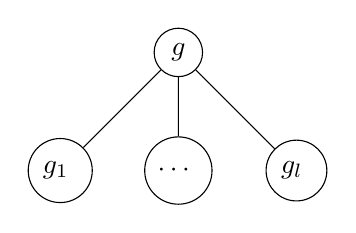
\begin{tikzpicture}[level distance=1.5cm,
  level 1/.style={sibling distance=1.5cm},
  every node/.style = {
  	shape=circle,
    draw,
    align=center,
    top color=white,
    bottom color=white
    }]
  \node {\( g \)}
    child {node { \( g_1 \) }}
    child {node { \( \cdots \) }}
    child {node { \( g_l \) }};
\end{tikzpicture}
\end{center}

For example, a circuit that encodes the function $f(a_1,a_2,a_3,a_4)=a_1a_2 +a_3a_4$ is 

\begin{center}
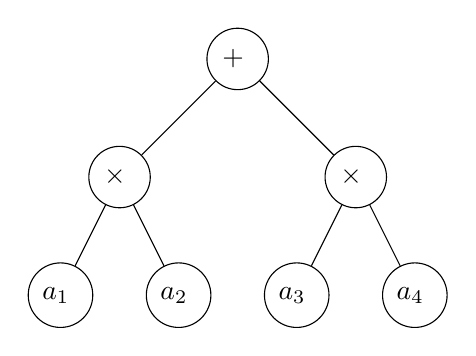
\begin{tikzpicture}[level distance=1.5cm,
  level 1/.style={sibling distance=3cm},
  level 2/.style={sibling distance=1.5cm},
  every node/.style = {
  	shape=circle,
    draw,
    align=center,
    top color=white,
    bottom color=white
    }
  ]
  \node { \( + \) }
    child { node { \( \times \) }
      child { node { \( a_1 \) } }
      child {node { \( a_2 \) } }
    }
    child { node { \( \times \) }
      child { node { \( a_3 \) } }
      child { node { \( a_4 \) } }
    };
\end{tikzpicture}
\end{center}

We can simulate the polynomial $x^2+xy$ by doing $f(A)$ where $A=[x \hspace{1ex} x \hspace{1ex} x \hspace{1ex} y]^*$. The main idea is to traverse the circuit top down in a depth first search way and store visited gates in a stack and its corresponding current values in another stack, and aggregate in the iterations according to the gate type.

For a stack $S$, the operations are standard:

\begin{itemize}
	\item $\push{S}{s}$: pushes $s$ into $S$.
	\item $\pop{S}$: pops the top element.
	\item $\getsize{S}$: the length of the stack.
	\item $\gettop{S}$: the top element in the stack.
\end{itemize}

For the pseudo-code, $\cG$ and $\cV$ denote stacks of gates and values, respectively. The property that holds during the simulation is that the value in $\cV[i]$ is the value that $\cG[i]$ currently outputs. The algorithm ends with $\cG=\left[ g_{\texttt{root}}\right]$ and $\cV=\left[ v_{\texttt{root}}\right]$ after traversing the circuit, and returns $v_{\texttt{root}}$

During the evaluation algorithm there will be two possible configurations of $\cG$ and $\cV$.

\begin{enumerate}
	\item $\getsize{\cG} = \getsize{\cV} + 1$: this means that $\gettop{\cG}$ is a gate that we visit for the first time and we need to initialize its value.
	
	\item $\getsize{\cG} = \getsize{\cV}$: here $\gettop{\cV}$ is the value of evaluating the circuit in gate $\gettop{\cG}$. Therefore, we need to aggregate the value $\gettop{\cV}$ to the parent gate of $g$.
\end{enumerate}

We assume the circuit has input gates, $+, \times$-gates and allow constant $1$-gate.

The idea is to traverse the circuit top down in a depth first search way. For example, in the circuit $f(a_1,a_2,a_3,a_4)=a_1a_2 +a_3a_4$ above, we would initialize the output gate value as $0$ because it is a $+$ gate, so $\cG=\lbrace +\rbrace$, $\cV=\lbrace 0\rbrace$. Then stack the left $\times$ gate to $\cG$, stack its initial value (i.e. $1$) to $\cV$. Now stack $a_1$ to $\cG$ and its value (i.e. $a_1$) to $\cV$. Since we are on an input gate we pop the gate and value pair off of $\cG$ and $\cV$ respectively, aggregate $a_1$ to $\gettop{\cV}$ and continue by stacking the $a_2$ gate to $\cG$. We pop $a_2$ off of $\cV$ (and its gate off of $\cG$) and aggregate its value to $\gettop{\cV}$. We pop and aggregate the value of the left $\times$ gate to $\gettop{\cV}$ (the root value). Then continue with the right $\times$ gate branch similarly.

For the pseudo-code, we supply ourselves with the following functions:

\begin{itemize}
	\item[--] $\isplus{g}$: true if and only if $g$ is a $+$-gate.
	\item[--] $\isprod{g}$: true if and only if $g$ is a $\times$-gate.
	\item[--] $\isone{g}$: true if and only if $g$ is a $1$-gate.
	\item[--] $\isinput{g}$: true if and only if $g$ is an input gate.
	\item[--] $\getfirst{g}$: outputs the first child of $g$.
	\item[--] $\getinput{g}$: outputs $A[i]$ when $g$ is the $i$-th input.
	\item[--] $\isnotlast{g_1}{g_2}$: true if and only if $g_2$ is not the last child gate of $g_1$.
	\item[--] $\nextgate{g_1}{g_2}$: outputs the next child gate of $g_1$ after $g_2$.
	\item[--] $\getroot$: outputs the root gate of the circuit.
\end{itemize}

The corresponding $\lbrace 0,1 \rbrace^n\rightarrow\lbrace 0,1 \rbrace^n$ functions are:

\begin{itemize}
	\item[--] $\isplus{g}$: $1$ if and only if $g$ is a $+$-gate.
	\item[--] $\isprod{g}$: $1$ if and only if $g$ is a $\times$-gate.
	\item[--] $\isone{g}$: $1$ if and only if $g$ is a $1$-gate.
	\item[--] $\isinput{g}$: $1$ if and only if $g$ is an input gate.
	\item[--] $\getfirst{g}$: outputs the $\texttt{id}$ of the first child of $g$.
	\item[--] $\getinput{g}$: outputs $e_i$ where the $i$-th input gate of $A$ is encoded by $g$.
	\item[--] $\isnotlast{g_1}{g_2}$: $1$ if and only if $g_2$ is not the last child gate of $g_1$.
	\item[--] $\nextgate{g_1}{g_2}$: outputs the $\texttt{id}$ of the next child gate of $g_1$ after $g_2$.
	\item[--] $\getroot$: outputs the $\texttt{id}$ of the root gate of the circuit.
\end{itemize}

The previous functions are all definable by an $L$-transducer and can be defined from the $L$-transducer of $f$. Then, by proposition \ref{prop:transducer}, for each of these functions there is a \langfor expression that simulates them.

Now, we give the pseudo-code of the top-down evaluation. We define the functions $Initialize$ (algorithm \ref{alg:init_code}), $Aggregate$ (algorithm \ref{alg:agg_code}) and $Evaluate$ (algorithm \ref{alg:eval_code}). The main algorithm is $Evaluate$.

\begin{algorithm}
\caption{Initialize (pseudo-code)}\label{alg:init_code}
\begin{algorithmic}[1]
\Function{Initialize}{$\cG, \cV, A$}\Comment{The stacks and input. Here, $\getsize{\cG} =  \getsize{\cV} + 1$}
	\If{$\isplus{\gettop{\cG}}$}
		\State $\push{\cV}{0}$
		\State $\push{\cG}{\getfirst{\gettop{\cG}}}$
	\ElsIf{$\isprod{\gettop{\cG}}$}
		\State $\push{\cV}{1}$
		\State $\push{\cG}{\getfirst{\gettop{\cG}}}$
	\ElsIf{$\isone{\gettop{\cG}}$}
		\State $\push{\cV}{1}$
	\ElsIf{$\isinput{\gettop{\cG}}$}
		\State $\push{\cV}{A\left[ \getinput{\gettop{\cG}} \right]}$
	\EndIf
	\State \textbf{return} $\cG, \cV$
\EndFunction
\end{algorithmic}
\end{algorithm}

\begin{algorithm}
\caption{Aggregate (pseudo-code)}\label{alg:agg_code}
\begin{algorithmic}[1]
\Function{Aggregate}{$\cG, \cV$}\Comment{Here, $\getsize{\cG} =  \getsize{\cV}$}
	\State $g = \pop{\cG}$
	\State $v = \pop{\cV}$
	\If{$\isplus{\gettop{\cG}}$}
		\State $\gettop{\cV} = \gettop{\cV} + v$
	\ElsIf{$\isprod{\gettop{\cG}}$}
		\State $\gettop{\cV} = \gettop{\cV} \cdot v$
	\EndIf
	\If{$\isnotlast{\gettop{\cG}}{g}$}
		\State $\push{\cG}{\nextgate{\gettop{\cG}}{g}}$
	\EndIf
	\State \textbf{return} $\cG, \cV$
\EndFunction
\end{algorithmic}
\end{algorithm}

\begin{algorithm}
\caption{Evaluate (pseudo-code)}\label{alg:eval_code}
\begin{algorithmic}[1]
\Function{Evaluate}{$A$}\Comment{Input $ n\times 1$ vector $A$. Here, $\cG$ and $\cV$ are empty}
	\State $\push{\cG}{\getroot}$
	\While{$\getsize{\cG}\neq 1$ or $\getsize{\cV}\neq 1$}
		\If{$\getsize{\cG}\neq \getsize{V}$}
			\State $(\cG,\cV) := \texttt{Initialize}(\cG,\cV,A)$
		\Else
			\State $(\cG,\cV):= \texttt{Aggregate}(\cG,\cV)$
		\EndIf
	\EndWhile
	\State \textbf{return} $\gettop{\cV}$
\EndFunction
\end{algorithmic}
\end{algorithm}

The $Evaluate$ algorithm gives us the output of the circuit. Note that after each iteration it either holds that $\getsize{\cG} =  \getsize{\cV} + 1$ or $\getsize{\cG} =  \getsize{\cV}$. Furthermore, when we start we have $\getsize{\cG}=1$ and $\getsize{\cV}=0$. The condition $\getsize{\cG}= 1$ and $\getsize{\cV}=1$ holds only when we have traversed all the circuit, and the value in $\gettop{\cV}$ is the value that the root of the circuit outputs after its computation.

Next, we show how to encode this algorithm in $\langfor$.

Let $n_0\in\mathbb{N}$ be big enough for $\star$ to hold and let $n\geq k$. Hence, the number of gates (values) is bounded by $n^k$ and we need $k\log (n)$ bits to encode the id of each gate.

To simulate the two stacks $\cG$ and $\cV$ we keep a matrix $X$ of dimensions $n \times n$.

\begin{itemize}
	\item Column $n$ will store a canonical vector that marks the top of stack $V$ (values).
	\item Column $n-1$ will store a canonical vector that marks the top of stack $G$ (gates).
	\item Column $n-2$ is the stack of values where $X[1, n-2]$ is the bottom of the stack.
	\item Columns $1$ to $n-3$ are the stack of gates.
\end{itemize}

If we have $j$ gates in the stack and currently $\getsize{\cG}=\getsize{\cV}$ then $X$ would look like:

\[
X = \begin{bmatrix}
    \texttt{id}_1 & v_1 & 0 & 0 \\
    \texttt{id}_2 & v_2 & 0 & 0 \\
    \vdots & \vdots & \vdots & \vdots \\
    \texttt{id}_j & v_j & 1 & 1 \\
    0 & 0 & 0 & 0 \\
    \vdots & \vdots & \vdots & \vdots \\
     0 & 0 & 0 & 0
\end{bmatrix}.
\]

Since $n\geq n_0$, $(\star)$ holds and thus we never use more than $n-3$ bits to encode an $\texttt{id}$ and $j\leq n$ given that we never keep more gates than the depth of the tree. As a consequence, we never keep more than $n$ values either.

We make a series of definitions to make the notation more clear.

Let $e_i$ be the $i$-th canonical vector. $S$ and $P$ denote the successor and predecessor matrices respectively, such that

\[
  			S\cdot e_i=\begin{cases}
               e_{i+1} \text{ if } i\leq n \\
               \mathbf{0} \text{ otherwise }
            \end{cases}
\]

\[
  			P\cdot e_i=\begin{cases}
               e_{i-1} \text{ if } i\geq n \\
               \mathbf{0} \text{ otherwise }
            \end{cases}
\]

We write $e_{min}$ for the first canonical vector and $e_{max}$ for the last canonical vector. For any $i$ we write 
\begin{align*}
	e_{min+i} &= S^i\cdot e_{min} \\
	e_{max+i} &= P^i\cdot e_{max}
\end{align*}

We use the extra $\lbrace 0,1 \rbrace^n\rightarrow\lbrace 0,1 \rbrace^n$ functions that have a $\langfor$ translation:

\[
  			min(e)=\begin{cases}
               1 \text{ if } e=e_{min} \\
               0 \text{ otherwise }
             \end{cases}
\]

\[
  			max(e)=\begin{cases}
               1 \text{ if } e=e_{max} \\
               0 \text{ otherwise }
             \end{cases}
\]

\[
  			less(e_i,e_j)=\begin{cases}
               1 \text{ if } i\leq j \\
               0 \text{ otherwise }
             \end{cases}
\]

When used in $\langfor$ these functions output $[0]$ and $[1]$.

Now 
\begin{align*}
	e_{V}&:=e_{max-2} \\
	e_{G_{top}}&:=e_{max-1} \\
	e_{V_{top}}&:=e_{max}
\end{align*}

For a canonical vector, let $$\Iden{e_i}:=\ssum v. less(v,e_i)\cdot (v\cdot v^*).$$ This matrix has ones in the diagonal up to position $i$ marked by $e_{i}$. We define the following sub-matrices of $X$:
\begin{align*}
	V_{top} &:= X\cdot e_{V_{top}} \\
	V &:= \Iden{V_{top}} \cdot X \cdot e_v \\
 	G_{top} &:=X\cdot e_{G_{top}} \\
 	G &:= \Iden{G_{top}}\cdot X \cdot \Iden{e_{max-3}}
\end{align*}

For example, if we are in a step where $\getsize{\cG}=\getsize{\cV} + 1$ then

\[
X = \begin{bmatrix}
    \texttt{id}_1 & v_1 & 0 & 0 \\
    \texttt{id}_2 & v_2 & 0 & 0 \\
    \vdots & \vdots & \vdots & \vdots \\
    \texttt{id}_{j-1} & v_{j-1} & 0 & 1 \\
    \texttt{id}_j & 0 & 1 & 0 \\
    0 & 0 & 0 & 0 \\
    \vdots & \vdots & \vdots & \vdots \\
     0 & 0 & 0 & 0
\end{bmatrix}, 
G = \begin{bmatrix}
    \texttt{id}_1  \\
    \texttt{id}_2 \\
    \vdots   \\
    \texttt{id}_{j-1} \\
    \texttt{id}_j \\
    0 \\
    \vdots \\
     0 
\end{bmatrix}, 
V = \begin{bmatrix}
    v_1  \\
    v_2 \\
    \vdots   \\
    v_{j-1} \\
    0 \\
    0 \\
    \vdots \\
     0 
\end{bmatrix}, 
G_{top} = \begin{bmatrix}
    0  \\
    0 \\
    \vdots   \\
    0 \\
    1 \\
    0 \\
    \vdots \\
     0 
\end{bmatrix}, 
V_{top} = \begin{bmatrix}
    0  \\
    0 \\
    \vdots   \\
    1 \\
    0 \\
    0 \\
    \vdots \\
     0 
\end{bmatrix}
\]

Here, $V$ is a vector encoding the stack of values in $X$ and $G$ is a matrix encoding the stack of gates in $X$. Note that what is \textit{over} the top of the stacks is always set to zero due to $\Iden{G_{top}}$ and $\Iden{V_{top}}$.

To set the initial state (algorithm \ref{alg:eval_code} line 2) we define the $\langfor$ expression: $$\text{START}:= e_{min}\cdot \getroot^* + e_{min}\cdot e_{G_{top}}^*.$$
For the initialize step, we define the $\langfor$ expressions: INIT${\_}$PLUS (algorithm \ref{alg:init_code}, lines 2, 3, 4), INIT${\_}$PROD (algorithm \ref{alg:init_code}, lines 5, 6, 7), CONST (algorithm \ref{alg:init_code}, lines 8, 9) and INPUT (algorithm \ref{alg:init_code}, lines 10, 11):

\begin{align*}
	\text{INIT{\_}PLUS} &:= \isplus{G^*\cdot G_{top}}\odot \left[ G + S\cdot G_{top} \cdot \getfirst{G^*\cdot G_{top}}^*  + S\cdot G_{top}\cdot e_{G_{top}}^* +V\cdot e_{V} + S\cdot V_{top}\cdot e_{V_{top}}^* \right] \\
	\text{INIT{\_}PROD} &:= \isprod{G^*\cdot G_{top}}\odot \left[ G + S\cdot G_{top} \cdot \getfirst{G^*\cdot G_{top}}^* + S\cdot G_{top}\cdot e_{G_{top}}^* +(V + S\cdot v_{top})\cdot e_{V} + S\cdot V_{top}\cdot e_{V_{top}}^* \right] \\
	\text{CONST} &:= \isone{G^*\cdot G_{top}}\odot \left[ G + (V + S\cdot v_{top})\cdot e_{V} + S\cdot V_{top}\cdot e_{V_{top}}^* \right] \\
	\text{INPUT} &:= \isinput{G^*\cdot G_{top}}\odot \left[ G + \left(V + \left( A^* \cdot \getinput{G^*\cdot G_{top}} \cdot S\cdot V_{top} \right)\right)\cdot e_{V} + S\cdot V_{top}\cdot e_{V_{top}}^* \right]
\end{align*} 

Here, $G^*\cdot G_{top}$ is to get the current id in the top of the stack. In INIT${\_}$PLUS we get the current stack $G$, we add $S\cdot G_{top} \cdot \getfirst{G^*\cdot G_{top}}^*$ which is an $n\times n$ matrix with the first child of $G^*\cdot G_{top}$ in the next row. Then $S\cdot G_{top}\cdot e_{G_{top}}^*$ adds $S\cdot G_{top}$ to the $n-1$ column to mark the gate we added as the top. Next, we do the same with the values by adding $V\cdot e_{V} + S\cdot V_{top}\cdot e_{V_{top}}^*$.

The $\langfor$ expression equivalent to algorithm \ref{alg:init_code} is $$\text{INIT}:=\text{INIT{\_}PLUS}+\text{INIT{\_}PROD}+\text{CONST}+\text{INPUT}.$$

The idea is to return the matrix for the next iteration. Recall that here $\getsize{\cG}=\getsize{\cV} + 1$. So, when the operation is INPUT or CONST, if we start with

\[
\begin{bmatrix}
    \texttt{id}_1 & v_1 & 0 & 0 \\
    \texttt{id}_2 & v_2 & 0 & 0 \\
    \vdots & \vdots & \vdots & \vdots \\
    \texttt{id}_{j-1} & v_{j-1} & 0 & 1 \\
    \texttt{id}_j & 0 & 1 & 0 \\
    0 & 0 & 0 & 0 \\
    \vdots & \vdots & \vdots & \vdots \\
     0 & 0 & 0 & 0
\end{bmatrix}, \text{ then we return }
\begin{bmatrix}
    \texttt{id}_1 & v_1 & 0 & 0 \\
    \texttt{id}_2 & v_2 & 0 & 0 \\
    \vdots & \vdots & \vdots & \vdots \\
    \texttt{id}_{j-1} & v_{j-1} & 0 & 0 \\
    \texttt{id}_j & v_j & 1 & 1 \\
    0 & 0 & 0 & 0 \\
    \vdots & \vdots & \vdots & \vdots \\
     0 & 0 & 0 & 0
\end{bmatrix}.
\]

When the operation is INIT{\_}PLUS or INIT{\_}PROD, if we start with 

\[
\begin{bmatrix}
    \texttt{id}_1 & v_1 & 0 & 0 \\
    \texttt{id}_2 & v_2 & 0 & 0 \\
    \vdots & \vdots & \vdots & \vdots \\
    \texttt{id}_{j-1} & v_{j-1} & 0 & 1 \\
    \texttt{id}_j & 0 & 1 & 0 \\
    0 & 0 & 0 & 0 \\
    0 & 0 & 0 & 0 \\
    \vdots & \vdots & \vdots & \vdots \\
     0 & 0 & 0 & 0
\end{bmatrix}, \text{ then we return }
\begin{bmatrix}
    \texttt{id}_1 & v_1 & 0 & 0 \\
    \texttt{id}_2 & v_2 & 0 & 0 \\
    \vdots & \vdots & \vdots & \vdots \\
    \texttt{id}_{j-1} & v_{j-1} & 0 & 0 \\
    \texttt{id}_j & v_j & 0 & 1 \\
    \texttt{id}_{j+1} & 0 & 1 & 0 \\
    0 & 0 & 0 & 0 \\
    \vdots & \vdots & \vdots & \vdots \\
     0 & 0 & 0 & 0
\end{bmatrix}.
\]


For the aggregate expression (algorithm \ref{alg:agg_code}) we do the following. Let $$\pondIden{e_i}{c}=\ssum v. (v^*\cdot e_i)\cdot c\cdot v\cdot v^* + (1-v^*\cdot e_i)\cdot v \cdot v^*,$$ namely, it is the identity with $c$ in position $(i,i)$.

We define the expressions: AGG${\_}$PLUS (algorithm \ref{alg:agg_code}, lines 4, 5), AGG${\_}$PROD (algorithm \ref{alg:agg_code}, lines 6, 7),  IS${\_}$NOT${\_}$LAST (algorithm \ref{alg:agg_code}, lines 8, 9), IS${\_}$LAST and POP:

\begin{align*}
	\text{POP} &:= \Iden{P\cdot G_{top}}\cdot G + P\cdot V_{top}\cdot e_{V_{top}}^*  \\
	\text{AGG{\_}PLUS} &:= \isplus{G^* \cdot \left( P \cdot G_{top}\right)} \odot \left[ \left( \Iden{P\cdot V_{top}} \cdot V + \left( V^* \cdot V_{top} \right)\left( P\cdot V_{top} \right)\right) \cdot e_{V}^* \right] \\
	\text{AGG{\_}PROD} &:= \isprod{G^* \cdot \left( P \cdot G_{top}\right)} \odot \left[ \left( \pondIden{P\cdot V_{top}}{V^* \cdot V_{top}} \cdot \Iden{P\cdot V_{top}} \cdot V \right) \cdot e_{V}^* \right] \\
	\text{IS{\_}NOT{\_}LAST} &:= \isnotlast{G^* \cdot \left( P \cdot G_{top}\right)}{G^* \cdot G_{top}} \odot \left[  G_{top} \cdot \nextgate{G^* \cdot \left( P\cdot G_{top} \right) }{G^* \cdot G_{top}} + G_{top}\cdot e_{G_{top}}^* \right] \\
	\text{IS{\_}LAST} &:= \left( 1 - \isnotlast{G^* \cdot \left( P \cdot G_{top}\right)}{G^* \cdot G_{top}} \right)\odot \left[ \left( P\cdot G_{top} \right) \cdot e_{G_{top}}^* \right]
\end{align*}

The $\langfor$ expression equivalent to algorithm \ref{alg:agg_code} is $$\text{AGG}:=\text{POP} + \text{AGG{\_}PLUS}+\text{AGG{\_}PROD}+\text{IS{\_}NOT{\_}LAST}+\text{IS{\_}LAST}.$$

The $Evaluate$ method (algorithm \ref{alg:eval_code}) is defined as follows:

\begin{align*}
	\text{EVAL}&[A]= \\
	&e_{min}^* \cdot \ffor{X}{v_1, \ldots, v_k}: \big\lbrace \\
	&\left( \sprod_{i=1}^k min(v_i)\right) \odot START + \\
	&\left( 1- \sprod_{i=1}^k min(v_i)\right) \odot \left( \left(1 - min(G_{top})\cdot min(V_{top}) \right) \odot \left[ \left( 1 - G_{top}^*\cdot V_{top} \right) \odot \text{INIT} + \left(  G_{top}^*\cdot V_{top} \right) \odot \text{AGG} \right] + min(G_{top})\odot min(V_{top})\odot X\right) \\ 
	&\big\rbrace \cdot e_{V}
\end{align*}

Note that the $ \texttt{for}$-expression does the evaluation. The final output is in $X[1,max-2]$, we extract this value by multiplying the final result as $e_{min}^*\cdot [\texttt{for}(\ldots )]\cdot e_{V}$.

Finally, we need to take care of all $n<n_0$, where $(\star)$ does not necessarily hold. For any $i$, let: $$\text{Eval}[i,A]:= \text{ the } 1\times 1 \text{ matrix with the value of the polynomial } f(A) \text{ when } n=i.$$

Then we define: $$f(A)=\ssum_{i=0}^{n_0-1}(e_{min+1}\cdot e_{max}^*)\odot \text{EVAL}[i,A] + \left( (S^{n_0}\cdot e_{min})^*\cdot \ones (e_{min}) \right)\odot \text{EVAL}[A].$$ Above, $(e_{min+1}\cdot e_{max}^*)$ checks if the dimension is equal to $i$, and $(S^{n_0}\cdot e_{min})^*\cdot \ones (e_{min})$ checks if the dimension is greater or equal than $n_0$.













\section{Logspace Stuff}

\section*{Simulating Logspace Turing machine on input $o^n$.}

We are given a logspace Turing Machine $T=\left(Q,\{0\},\ell,\rhd,\lhd,\Delta,q_0,q_m\right)$ where $Q=\{q_1,\ldots,q_m\}$ are the states, $\ell$ denotes the number of heads, $q_0$ and $q_m$ denote initial and final state, respectively, $\{0\}$ is the tape alphabet, and $\rhd$ and $\lhd$ are special symbols denoting the beginning and the end of the tape, respectively. Finally,
$\Delta=(\Delta_Q,\Delta_1,\ldots,\Delta_\ell)$ is the transition function of $T$, where $\Delta_Q:Q\times \{\rhd,0,\lhd\}^\ell\mapsto Q$ and for $i\in[\ell]$,
$\Delta_i:Q\times  \{\rhd,0,\lhd\}^\ell\mapsto\{\gets,\to\}$. In other words, when $T$ is in state $q$ and the $\ell$ heads read symbols $b_1,\ldots,b_\ell$, $\Delta_Q(q,b_1,\ldots,b_\ell)$ indicates to which state $T$ will transition, and moreover, $\Delta_i(q,b_1,\ldots,b_\ell)$ says in which direction (left or right) the $i$th head will move. We assume that when $T$ is in the initial state $q_0$ all heads point to the first position (i.e., they all read symbol $\rhd$). 

In our setting, the tape contents will always be of the form $w_n:=\rhd 0^n \lhd$ for some $n\in\mathbb{N}$. As usual, $T$ cannot move beyond the begin and end markers, $\rhd$ and $\lhd$, respectively. We assume that $T$ accepts or rejects the input $w_n$ using $\mathcal{O}(n^k)$ steps. In other words, there exists a constant $c$ such that $T$ runs in at most $cn^k$ steps. For simplicity, we assume that $T$ runs for at most $n^{k+1}$ steps. For technical reasons, that will become clear below, we assume that once $T$ reaches the final state $q_m$, $T$ will further transition but only to the state $q_m$. That is, $\Delta$ contains transitions that make $T$ loop in $q_m$.

\begin{proposition}
Given a logspace Turing machine $T$ with $m$ states, $\ell$ heads and which runs on $w_n=\rhd 0^n \lhd$ in time $n^{k+1}$, for $n\in\mathbb{N}$, there exists (i)~a $\mathsf{MATLANG}$ 
schema $\mathcal{S}=(\mathcal{M},\textsf{size})$ where $\mathcal{M}$ consists matrix variables\footnote{We also need a finite number of auxiliary variables, these will be specified in the proof.} $X_1,\ldots,X_m,Y_1,\ldots,Y_\ell, v_1,\ldots,v_{k+1}$ and $w$ with
$\mathsf{size}(V)=\alpha\times 1$ for all $V\in\mathcal{M}$ and $V\neq w$ and $\mathsf{size}(w)=1\times 1$; and (ii)~a $\mathsf{MATLANG}$ expression $e_T$ over $\mathcal{S}$ such that for the instance $I=(\mathcal{D},\textsf{mat})$ over $\mathcal{S}$ with $\mathcal{D}(\alpha)=n+2$ and $\mathsf{mat}(V)=\left(\begin{smallmatrix}0\\
0\\\vdots\\0\end{smallmatrix}\right)$ for all $V\in\mathcal{M}$ and
$\mathsf{mat}(w)=[0]$, we have that 
$e_T(I)=[1]$ if $T$ accepts $w_n$ and  $e_T(I)=[0]$ otherwise.
\end{proposition}
\begin{proof}
We start by explaining the semantics of the matrix variables in $\mathcal{M}$. The variables $X_1,\ldots,X_m,Y_1,\allowbreak\ldots,Y_\ell$ will be used inside for loops and will be updated using \textsf{MATLANG} expressions. Initially, all these matrix variables are instantiated with the zero column vector, as described by the instance $I$. 

With each state $q_i\in Q$ we associate matrix variable $X_i$.
Then, $T$ is in state $q_i$ when
 $X_i=\left(\begin{smallmatrix}1\\
0\\\vdots\\0\end{smallmatrix}\right)$, otherwise $X_i=\left(\begin{smallmatrix}0\\
0\\\vdots\\0\end{smallmatrix}\right)$.	Similarly, with each head $i\in[\ell]$ we
associate matrix variable $Y_i$. When the $i$th head points at position $j$ in $w_n$,
then $Y_i=\mathsf{e}_j$, i.e., it is the $j$th canonical column vector. We remark that since the dimensions is $n+2$ and $T$ cannot change the input word $w_n$, the $n+2$ canonical vectors suffice to indicate all positions in $w_n$ (which is of length $n+2$).

The variables $v_1,\ldots,v_{k+1}$ represent $k+1$ canonical vectors  which are use to iterate in for loops. By iterating over then, we can perform $(n+2)^{k+1}$ iterations, which suffices for simulating the $n^{k+1}$ steps used by $T$ on input $w_n$.

Finally, the variable $w$ is used for the output of $e_T$. It contains a scalar and will hold $1$ if $w_n$ is accepted by $T$ and $0$ otherwise.

The expression $e_T$ uses some subexpressions in $\mathsf{MATLANG}$ which use some auxiliary variables.
As a consequence, $e_T$ is an expression defined over an extended schema $\mathcal{S}'$. Hence, the instance $I$ in the statement of the Proposition is in fact an instance $I'$ of $\mathcal{S}'$ which
coincides with $I$ on $\mathcal{S}$ and in which the auxiliary matrix variables are all instantiated with zero vectors or matrices, depending on their size.

We list the used subexpressions next and explicitly denote the auxiliary matrix variables:
\begin{itemize}
	% \item $\mathsf{max}(z,Z)$, an expression over auxiliary variables $z$ and $Z$ with $\mathsf{size}(z)=\mathsf{size}(Z)=\alpha\times 1$. On input $I'$ with
	% $\mathsf{mat}(z)=\mathsf{mat}(Z)$ the zero column vector of dimension $n+2$,
	%  $\mathsf{max}(I)=\mathbf{e}_{n+2}$.
	\item $\mathsf{pred}(z,Z,z',Z')$, and expression over auxiliary variables $z$, $z'$, $Z$ and $Z'$ with $\mathsf{size}(z)=\mathsf{size}(z')=\mathsf{size}(Z)=\alpha\times 1$ and $\mathsf{size}(Z')=\alpha\times\alpha$. On input $I'$ with 
	$\mathsf{mat}(z)=\mathsf{mat}(z')=\mathsf{mat}(Z)$ the zero column vector of dimension $n+2$, and $\mathsf{mat}(Z')$ the zero $(n+2)\times (n+2)$ matrix,
	 $\mathsf{pred}(I')$ returns an $(n+2)\times (n+2)$ matrix such that 
	 
	 $$\mathsf{pred}(I')\mathbf{e}_i:=\begin{cases} 
	 \mathbf{e}_{i-1} & \text{if $i>1$}\\
	 \mathbf{0} & \text{if $i=1$}.
	\end{cases}
	$$
	In other words, $\mathsf{pred}$ defines a predecessor relation among canonical vectors of dimension $n+2$.
	 \item $\mathsf{succ}(z,Z,z',Z')$, and expression over auxiliary variables $z$, $z'$, $Z$ and $Z'$ with $\mathsf{size}(z)=\mathsf{size}(z')=\mathsf{size}(Z)=\alpha\times 1$ and $\mathsf{size}(Z')=\alpha\times\alpha$. On input $I'$ with 
	$\mathsf{mat}(z)=\mathsf{mat}(z')=\mathsf{mat}(Z)$ the zero column vector of dimension $n+2$, and $\mathsf{mat}(Z')$ the zero $(n+2)\times (n+2)$ matrix,
	 $\mathsf{succ}(I')$ returns an $(n+2)\times (n+2)$ matrix such that 
	 
	 $$\mathsf{succ}(I')\mathbf{e}_i:=\begin{cases} 
	 \mathbf{e}_{i+1} & \text{if $i<n+2$}\\
	 \mathbf{0} & \text{if $i=n+2$}.
	\end{cases}
	$$
	In other words, $\mathsf{succ}$ defines a successor relation among canonical vectors.
	\item $\textsf{ismin}(v,z,Z,z',Z)$ with auxiliary variables $z$, $z'$, $Z$ and $Z'$ as before, and $v$ is one of the (vector) variables in $\mathcal{M}$. For an $(n+2)\times 1$ vector $\mathbf{v}$, on input $I'[v\gets \mathbf{v}]$	$$\mathsf{ismin}(I'[v\gets\mathbf{v}]):=\begin{cases} 1 & \text{if $\mathbf{v}=\mathbf{e}_1$}\\
		0 & \text{otherwise}.
		\end{cases}$$
	\item $\textsf{ismax}(v,z,Z,z',Z)$ with auxiliary variables $z$, $z'$, $Z$ and $Z'$ as before, and 
	and $v$ is one of the (vector) variables in $\mathcal{M}$. For an $(n+2)\times 1$ vector $\mathbf{v}$, on input $I'[v\gets \mathbf{v}]$
	
	$$\mathsf{ismax}(I'[v\gets\mathbf{v}]):=\begin{cases} 1 & \text{if $\mathbf{v}=\mathbf{e}_{n+2}$}\\
		0 & \text{otherwise}.
		\end{cases}$$
	\item $\mathsf{min}(z,Z,z',Z',z'',Z'')$, an expressions with
	auxiliary variables $z$, $z'$, $z''$, $Z$, $Z'$ and $Z''$ with $\mathsf{size}(z)=\mathsf{size}(z')=\mathsf{size}(z'')=\mathsf{size}(Z)=\mathsf{size}(Z'')\alpha\times 1$ and $\mathsf{size}(Z')=\alpha\times\alpha$. On input $I'$ with 
	matrix variables instantiated with zero vectors (or matrix for $Z'$),
 	 $\mathsf{min}(I')=\mathbf{e}_1$. 
	 		\item We additionally define, based on the previous expressions, 
			$$\mathsf{test}_b(v,z,Z,z',Z'):=\begin{cases} \mathsf{ismin}(v,z,Z,z,Z') & \text{if $b=\rhd$}\\
     \mathsf{ismax}(v,z,Z,z,Z') & \text{if $b=\lhd$}\\
	 (1-\mathsf{ismin}(v,z,Z,z',Z'))(1-\mathsf{ismax}(v,z,Z,z',Z')) & \text{if $b=0$}.
		\end{cases}.$$
	When evaluated on $I'[v\gets\mathbf{v}]$, $\mathsf{test}_b(I'[v\gets\mathbf{v}])$ will be $1$ when either
	$\mathbf{v}=\mathbf{e}_{1}$ and $b=\rhd$ (first position)
	$\mathbf{v}=\mathbf{e}_{n+2}$ and $b=\lhd$ (last position),
	$\mathbf{v}\neq \mathbf{e}_{1}$ and $\mathbf{v}\neq \mathbf{e}_{n+2}$  and $b=0$ (not first or last position). We use this expression below to check whether the heads are consistent with the symbols on the tape.
	
	
 \item Finally, we define
 $$
 \mathsf{move}_d(z,Z,z',Z'):=\begin{cases}
 e_{\mathsf{pred}}(z,Z,z',Z) & \text{if $d=\gets$}\\
  e_{\mathsf{succ}}(z,Z,z',Z) & \text{if $d=\to$}. 
 \end{cases},
 $$
 $\mathsf{move}_d(I')$ will simply return the predecessor matrix when $d=\gets$ and the successor matrix when $d=\to$. This expression will be used to move the heads.
\end{itemize}
We thus see that we only need $z,z',z'',Z,Z',Z''$ as auxiliary variables and these can be re-used for every occurrence of the subexpressions in $e_T$. From now one, we omit the auxiliary variables from the description of $e_T$.

We define the expression $e_T$, as follows\footnote{In the expression I uses $;w$ to indicate the output variable. That is, the for loops updates all instances for $X_1,\ldots,X_m,Y_1,\ldots,Y_\ell$ and $w$, but the result of the expression is only what is in the instance corresponding to $w$. We can simulate this again if we allow constant dimensional canonical basis vectors in $\mathsf{MATLANG}$.}:
$$
e_T:= \mathsf{for\,} v_1,\ldots,v_{k+1},X_1,\ldots,X_m,Y_1,\ldots,Y_\ell; w.(e_w,e_{X_1},\ldots,e_{X_m},e_{Y_1},\ldots,e_{Y_\ell}),
$$
with 
\begin{align*}\allowdisplaybreaks
	e_w&:=\mathsf{ismin}(X_m)\\
	e_{X_1}&:=\left(\prod_{j=1}^{k+1} \textsf{ismin}(v_i)\right)\cdot\mathsf{min}
	+ \sum_{\substack{q,b_1,\ldots,b_\ell\\
	\Delta_Q(q,b_1,\ldots,b_\ell)=q_1}} \!\!\!\!\!\!\!\!\! \textsf{ismin}(X_q)\left(\prod_{j=1}^\ell \mathsf{test}_{b_j}(Y_j)\right)\mathsf{min}\\
	e_{X_i}&:= \sum_{\substack{q,b_1,\ldots,b_\ell\\
	\Delta_Q(q,b_1,\ldots,b_\ell)=q_i}}\!\!\!\!\!\!\!\!\! \textsf{ismin}(X_q)\left(\prod_{j=1}^\ell \mathsf{test}_{b_j}(Y_j)\right)\mathsf{min} \quad \text{for $i\neq 1$}\\
	e_{Y_i}&:=\left(\prod_{j=1}^{k+1} \textsf{ismin}(v_i)\right)\cdot\mathsf{min}
	+\sum_{\substack{q,b_1,\ldots,b_\ell\\
	\Delta_i(q,b_1,\ldots,b_\ell)=d}}\!\!\!\!\!\!\!\!\! \textsf{ismin}(X_q)\left(\prod_{j=1}^\ell \mathsf{test}_{b_j}(Y_j)\right)\mathsf{move}_d\cdot Y_i
\end{align*}

The correctness of $e_T$ is now readily verified. We do this by induction on the number of iterations in the for loop. We note that initially, all variables are assigned zero vectors and values (for $w$). 

At the start of the run of $T$, we are in state $q_1$ and all heads point to the first position. We argue that after the first 
iterations, i.e., when $v_i=\mathbf{e}_1$ for $i\in[k+1]$, we indeed have that $X_1=\mathbf{e_1}$, $X_j=\mathbf{0}$ for $j\neq 1$, and $Y_j=\mathbf{e}_1$ for $j\in[\ell]$. Indeed, in the expression for $e_{X_1}$ the test $\prod_{j=1}^{k+1} \textsf{ismin}(v_i)$ will return $1$ and hence $X_1$ is replaced by $\mathsf{min}=\mathbf{e}_1$. Since all $X_i$ are initially zero, $\mathsf{ismin}(X_i)$ evaluate to zero for all $i\in[m]$ so the second term in $e_{X_1}$ adds the zero vector to $\mathbf{e}_1$ and thus $X_1$ remains $\mathbf{e_1}$.
Similarly, $e_{X_j}$ for $j\neq 1$ will leave $X_j$ unchanged, so these remain zero vectors. For the head positions, a similar arguments shows that after the first iterations, all $Y_i$ are set of $\mathbf{e}_1$.

We next assume that up to a certain iteration $\kappa-1$, the matrix variables correctly encode a configuration of $T$ on $w_n$ and furthermore, this configuration is reachable from the initial configuration. We next show that this remains to hold in the $\kappa$th iteration.

By induction, there will be a single $X_i$ which is instantiated with $\mathbf{e}_1$. Let use assume that this $X_q$. All other $X_i$ are instantiated with the zero vector. Furthermore, $Y_j=\mathbf{e}_{i_j}$ for some $i_j\in[n+2]$. 

Suppose that
$\Delta_Q(q,b_{i_1},\ldots,b_{i\ell})=p$ and
$\Delta_j(q,b_{i_1},\ldots,b_{i\ell})=d_j$. Then, inspecting the expressions $e_{X_i}$, all $X_{q_i}$ with $q_i\neq p$ will be replaced by the zero vector. The reason is that for $X_i$ to be replaced by $\mathsf{min}$ (i.e., $\mathbf{e}_1$) when $T$ is in state $q$,
there must be a transition $\Delta_Q(q,b_{i_1}',\ldots,b_{i_\ell}')=q_i$
and such that the $b_{i_j}'$ corresponds to the positions encoded by
the $Y_i$'s. In particular, $b_{i_1},\ldots,b_{i\ell}$ and 
$b_{i_1}',\ldots,b_{i_\ell}'$ must have $\rhd$ and $\lhd$ at the same positions, and since the only remaining symbol is $0$, $b_{i_1},\ldots,b_{i\ell}$ and $b_{i_1}',\ldots,b_{i\ell}'$ must agree.
This in turn would imply that there are two possible states $p$ and $q_i$ from $q$ while reading $b_{i_1},\ldots,b_{i\ell}$. This is impossible since $T$ is deterministic.

If we next consider the expressions $e_{Y_i}$ for $i\in[\ell]$, then a similar argument shows that at most one of the terms in the second part in $e_{Y_i}$ can replace $Y_i$ with $\mathsf{move}_d\cdot Y_i$. By defining of $\mathsf{move}_d$ in terms of the predecessor or successor matrix (depending on whether $d=\gets$ or $d=\to$, respectively), and given that $Y_i$ corresponds to a canonical vector, say $\mathbf{e}_{i_s}$, then $\mathsf{move}_d\cdot Y_i$ will replace $Y_i$
with either $\mathbf{e}_{i_s-1}$ or  $\mathbf{e}_{i_s+1}$. We note that when $Y_i$ is $\mathbf{e}_1$ or $\mathbf{e}_{n+2}$, $d$ must necessarily be $\to$ or $\gets$, respectively, since $T$ does not move beyond the end markers. 

Hence, all combined we see that after the $\kappa$the iteration, $X_1,\ldots,X_m$ and $Y_1,\ldots,Y_\ell$ indeed correspond to the next configuration of $T$.

We now remark that $w$ will be zero unless in one of the iterations populates $X_m$ with $\mathbf{e}_{1}$, i.e., the $T$ is in the final state. By assumption, $T$ will continue to be in the final state from that point on, and thus after perform our $(n+2)^k$, $w$ will remain $1$. If no final state is encountered, $w$ remains $0$, as desired.
\end{proof}

\section*{Simulating Linear Space Functions}
We consider  deterministic Turing Machines  (TM) $T$ consisting of $\ell$ read-only input tapes, denoted by $R_1,\ldots,R_\ell$,
a work tape, denoted by $W$, and a write-only output tape, denoted by $O$. The TM $T$ has a set $Q$ of $m$
states, denoted by $q_0,\ldots,q_m$. We assume that $q_0$ is the initial state and $q_m$ is the accepting state.
The input and tape alphabet are $\Sigma=\{0,1\}$ and $\Gamma=\Sigma\cup\{\rhd,\lhd\}$, respectively. The special symbol $\rhd$ denotes the beginning of each of the tapes, the symbol $\lhd$ denotes the end of the $\ell$ input tapes. The transition function $\Delta$ is defined as usual, i.e., 
$\Delta:Q\times \Gamma^{\ell+2} \to Q\times \Gamma^{2}\times \{\leftarrow,\sqcup,\rightarrow\}^{\ell+2}$ such that $\Delta(q,(a_1,\ldots,a_{\ell},b,c))=\bigl(q',(b',c'),(\mathsf{d}_1,\ldots,\mathsf{d}_{\ell+2})\bigr)$ with $\mathsf{d}_i\in \{\leftarrow,\sqcup,\rightarrow\}$, means that when $T$ is in state $q$ and the $\ell+2$ heads on the tapes read symbols $a_1,\ldots,a_{\ell},b,c$, respectively, then $T$ transitions to state $q'$, writes $b',c'$ on the work and output tapes, respectively, at the position to which the work and output tapes' heads points at, and finally moves the heads on the tapes according $\mathsf{d}_1,\ldots,\mathsf{d}_{\ell+2}$. More specifically, $\leftarrow$  indicates a move to the left, 
$\rightarrow$ a move to the right, and finally, $\sqcup$ indicates that the head does not move.

We assume that $\Delta$ is defined such that it ensures that on none of the tapes, heads can move beyond the leftmost marker $\rhd$. Furthermore, the tapes $R_1,\ldots,R_\ell$ are treated as read-only the head cannot move beyond the end markers $\lhd$ on each of the input tapes. Similarly, $\Delta$ ensures that the output tape $O$ is write only, i.e., its head cannot move to the left.  We also assume that $\Delta$ does not change $\rhd$ or write $\lhd$ on the work and output tape.

A configuration of $T$ is defined in the usual way. That is, a configuration the input tapes is of the form
$\rhd w_1qw_2\lhd$ with $w_1,w_2\in\Sigma^*$ and represents that the current tape content is $\rhd w_1w_2\lhd$, $T$ is state $q$ and the head is position on the first symbol of $w_2$. Similarly, a configuration of the work and output tape are represented by $\rhd w_1qw_2$. A configuration of $T$ is consists of configurations for all tapes. Given two configurations $c_1$ and $c_2$, we say that $c_1$
transitions to $c_2$ if $c_2$ is the result of applying the transition function based on the information in $c_1$. Given $\ell$ input words $w_1,\ldots,w_\ell\in\Sigma^*$, the initial configuration is given by
 $\bigl(\rhd q_0 w_1\lhd,\rhd q_0 w_2\lhd,\ldots, \rhd q_0 w_\ell\lhd,\rhd q_0,\rhd q_0\bigr)$ and the accepting configuration is given by $\bigl(\rhd q_m w_1\lhd,\rhd q_m w_2\lhd,\ldots, \rhd q_m w_\ell\lhd,\rhd q_m,\rhd q_m w\bigr)$ for some $w\in\Sigma^*$. We say that $T$ computes the function $f:(\Sigma^*)^{\ell}\to\Sigma^*$ if for every $w_1,\ldots,w_\ell\in\Sigma^*$, $T$ transitions (transitively) from the initial configuration to the accepting configuration such that the configuration on the output tape is
 given by $\rhd q_m f(w_1,\ldots,w_\ell)$.

We assume that once $T$ reaches an accepting configuration it stays indefinitely in that configuration (i.e., it loops). We further assume that $T$ only reaches an accepting configuration when all its input
words have the same size. Furthermore, for every such input words, $T$ will reach an accepting configuration.


We say that $T$ is a \textit{linear space machine} when it reaches an accepting configuration 
on inputs of size $n$ by using $sn$ space on its work tape and additionally needs  $\mathcal{O}(n^k)$ steps to do so. A \textit{linear input-output function} is a function of the form $f=\bigcup_{n\geq 0} f_n:(\Sigma^n)^\ell\to\Sigma^n$. In other words, for every $\ell$ words of the same size $n$ it returns a word of size $n$. We say that a linear input-output function is a linear space input-output function if
there exists a linear space machine  $T$ that on input $w_1,\ldots,w_\ell\in\Sigma^n$ puts
$f_n(w_1,\ldots,w_\ell)$ on its the output tape when (necessarily) reaching an accepting configuration.

% We say that a function
% $f:\underbrace{\Sigma^n\times\cdots \times \Sigma^n}_{\text{$\ell$ times}}\to \Sigma^n$ is computable by a linear space machine $T$ if when $T$ is run on input $w_1,\ldots,w_\ell$ it halts and has $f(w_1,\ldots,w_\ell)$ on its output tape. We say that $f$ is a \textit{linear space poly function} if it is computable by a linear space TM $T$ which in addition runs in polynomial time, i.e., it hals in at most
% $\mathcal{O}(n^k)$ steps for a certain $k$ on any inputs $w_1,\ldots,w_\ell$ of size $n$.
\begin{proposition}
Let $f=\bigcup_{n\geq 0}f_n:(\Sigma^n)^\ell\to \Sigma^n$ be a linear space input-ouput function computed by a linear space  machine $T$ with $m$ states, $\ell$ input tapes, which consumes $sn$ space and runs in $\mathcal{O}(n^{k-1})$ time on inputs of size $n$. Then  exists (i)~a $\mathsf{MATLANG}$ 
schema $\mathcal{S}=(\mathcal{M},\textsf{size})$ where $\mathcal{M}$ consists matrix variables\footnote{We also need a finite number of auxiliary variables, these will be specified in the proof.} $Q_1,\ldots,Q_m,R_1,\ldots,R_\ell,H_1,\ldots,H_\ell,W_1,\ldots,W_s,H_{W_1},\ldots,H_{W_s},O,H_O, v_1,\ldots,v_{k}$  with
$\mathsf{size}(V)=\alpha\times 1$ for all $V\in\mathcal{M}$; and (ii)~a $\mathsf{MATLANG}$ expression $e_f$ over $\mathcal{S}$ such that for the instance $I=(\mathcal{D},\textsf{mat})$ over $\mathcal{S}$ with $\mathcal{D}(\alpha)=n$ and 
$$\mathsf{mat}(R_i)=\mathsf{vec}(w_i)\in \mathbb{R}^n\text{ and } \mathsf{mat}(Q_i)=\mathsf{mat}(H_i)=\mathsf{mat}(W_i)=\mathsf{mat}(H_{W_i})=\mathsf{mat}(O)=\mathsf{mat}(H_O)=[0]\in \mathbb{R}^n, 
$$
for words $w_1,\ldots,w_\ell\in\Sigma^n$ and such that $\mathsf{vec}(w_i)$ is the $n\times 1$-vector encoding the symbols in $w_i$, we have that $e_f(I)=\mathsf{vec}(f_n(w_1,\ldots,w_n))$.
\end{proposition}
\begin{proof}
We start by explaining the semantics of the matrix variables in $\mathcal{M}$. The variables $R_1,\ldots,R_\ell$ will hold the input vectors, $W_1,\ldots,W_s$ will hold the contents of the work
tape, and $O$ will hold the contents of the output tape. The vectors corresponding to the work and output tape are initially set to the zero vector.

 With each tape we associate a matrix variable encoding the position of the head. More specifically, $H_1,\ldots,H_\ell$ correspond to the input tape heads,
$H_{W_1},\ldots, H_{W_s}$ are the heads for the work tape (note that the size of work tape is $sn$ we encode this by $s$ tapes of size $n$), and $H_O$ is the head of the output tape. All these vectors are initialised with the zero vector. Later on, these vectors have will be zero except for the position to which the head points to, which will hold the value $1$.

%
% ,Y_1,\allowbreak\ldots,Y_\ell$ will be used inside for loops and will be updated using \textsf{MATLANG} expressions. Initially, all these matrix variables are instantiated with the zero column vector, as described by the instance $I$.
Furthermore, with each state $q_i\in Q$ we associate matrix variable $Q_i$.
Then, $T$ is in state $q_i$ when
 $Q_i=\left(\begin{smallmatrix}1\\
0\\\vdots\\0\end{smallmatrix}\right)$, otherwise $Q_i=\left(\begin{smallmatrix}0\\
0\\\vdots\\0\end{smallmatrix}\right)$.	

The variables $v_1,\ldots,v_{k}$ represent $k$ canonical vectors  which are use to iterate in for loops. By iterating over then, we can perform $(n)^{k}$ iterations, which suffices for simulating the $\mathcal{O}(n^{k-1})$ steps used by $T$ to reach an accepting configuration. (We recall that $T$ loops when reaching an accepting configuration.) In the following
we assume that $n$ is sufficiently large, say $n\geq N$, such that $T$ runs in at most $cn^{k-1}$ steps. We deal with
the finite number of cases $n<N$ later on.

The expression $e_f$ uses some subexpressions in $\mathsf{MATLANG}$ which use some auxiliary variables.
As a consequence, $e_f$ is an expression defined over an extended schema $\mathcal{S}'$. Hence, the instance $I$ in the statement of the Proposition is in fact an instance $I'$ of $\mathcal{S}'$ which
coincides with $I$ on $\mathcal{S}$ and in which the auxiliary matrix variables are all instantiated with zero vectors or matrices, depending on their size.

We list the used subexpressions next and explicitly denote the auxiliary matrix variables:
\begin{itemize}
	% \item $\mathsf{max}(z,Z)$, an expression over auxiliary variables $z$ and $Z$ with $\mathsf{size}(z)=\mathsf{size}(Z)=\alpha\times 1$. On input $I'$ with
	% $\mathsf{mat}(z)=\mathsf{mat}(Z)$ the zero column vector of dimension $n+2$,
	%  $\mathsf{max}(I)=\mathbf{e}_{n+2}$.
	\item $\mathsf{pred}(z,Z,z',Z')$, and expression over auxiliary variables $z$, $z'$, $Z$ and $Z'$ with $\mathsf{size}(z)=\mathsf{size}(z')=\mathsf{size}(Z)=\alpha\times 1$ and $\mathsf{size}(Z')=\alpha\times\alpha$. On input $I'$ with 
	$\mathsf{mat}(z)=\mathsf{mat}(z')=\mathsf{mat}(Z)$ the zero column vector of dimension $n$, and $\mathsf{mat}(Z')$ the zero $n\times n$ matrix,
	 $\mathsf{pred}(I')$ returns an $n\times n$ matrix such that 
	 
	 $$\mathsf{pred}(I')\mathbf{e}_i:=\begin{cases} 
	 \mathbf{e}_{i-1} & \text{if $i>1$}\\
	 \mathbf{0} & \text{if $i=1$}.
	\end{cases}
	$$
	In other words, $\mathsf{pred}$ defines a predecessor relation among canonical vectors of dimension $n$.
	 \item $\mathsf{succ}(z,Z,z',Z')$, and expression over auxiliary variables $z$, $z'$, $Z$ and $Z'$ with $\mathsf{size}(z)=\mathsf{size}(z')=\mathsf{size}(Z)=\alpha\times 1$ and $\mathsf{size}(Z')=\alpha\times\alpha$. On input $I'$ with 
	$\mathsf{mat}(z)=\mathsf{mat}(z')=\mathsf{mat}(Z)$ the zero column vector of dimension $n$, and $\mathsf{mat}(Z')$ the zero $n\times n$ matrix,
	 $\mathsf{succ}(I')$ returns an $n\times n$ matrix such that 
	 
	 $$\mathsf{succ}(I')\mathbf{e}_i:=\begin{cases} 
	 \mathbf{e}_{i+1} & \text{if $i<n$}\\
	 \mathbf{0} & \text{if $i=n$}.
	\end{cases}
	$$
	In other words, $\mathsf{succ}$ defines a successor relation among canonical vectors.
	\item $\textsf{ismin}(v,z,Z,z',Z)$ with auxiliary variables $z$, $z'$, $Z$ and $Z'$ as before, and $v$ is one of the (vector) variables in $\mathcal{M}$. For an $n\times 1$ vector $\mathbf{v}$, on input $I'[v\gets \mathbf{v}]$	$$\mathsf{ismin}(I'[v\gets\mathbf{v}]):=\begin{cases} 1 & \text{if $\mathbf{v}=\mathbf{e}_1$}\\
		0 & \text{otherwise}.
		\end{cases}$$
	\item $\textsf{ismax}(v,z,Z,z',Z)$ with auxiliary variables $z$, $z'$, $Z$ and $Z'$ as before, and 
	and $v$ is one of the (vector) variables in $\mathcal{M}$. For an $n\times 1$ vector $\mathbf{v}$, on input $I'[v\gets \mathbf{v}]$
	
	$$\mathsf{ismax}(I'[v\gets\mathbf{v}]):=\begin{cases} 1 & \text{if $\mathbf{v}=\mathbf{e}_{n+2}$}\\
		0 & \text{otherwise}.
		\end{cases}$$
	\item $\mathsf{min}(z,Z,z',Z',z'',Z'')$, an expressions with
	auxiliary variables $z$, $z'$, $z''$, $Z$, $Z'$ and $Z''$ with $\mathsf{size}(z)=\mathsf{size}(z')=\mathsf{size}(z'')=\mathsf{size}(Z)=\mathsf{size}(Z'')\alpha\times 1$ and $\mathsf{size}(Z')=\alpha\times\alpha$. On input $I'$ with 
	matrix variables instantiated with zero vectors (or matrix for $Z'$),
 	 $\mathsf{min}(I')=\mathbf{e}_1$. 
	 		\item We additionally define, based on the previous expressions, 
			$$\mathsf{test}_b(v,z,Z,z',Z'):=\begin{cases} \mathsf{ismin}(v,z,Z,z,Z') & \text{if $b=\rhd$}\\
     \mathsf{ismax}(v,z,Z,z,Z') & \text{if $b=\lhd$}\\
	 (1-\mathsf{ismin}(v,z,Z,z',Z'))(1-\mathsf{ismax}(v,z,Z,z',Z')) & \text{if $b=0$}.
		\end{cases}.$$
	When evaluated on $I'[v\gets\mathbf{v}]$, $\mathsf{test}_b(I'[v\gets\mathbf{v}])$ will be $1$ when either
	$\mathbf{v}=\mathbf{e}_{1}$ and $b=\rhd$ (first position)
	$\mathbf{v}=\mathbf{e}_{n+2}$ and $b=\lhd$ (last position),
	$\mathbf{v}\neq \mathbf{e}_{1}$ and $\mathbf{v}\neq \mathbf{e}_{n+2}$  and $b=0$ (not first or last position). We use this expression below to check whether the heads are consistent with the symbols on the tape.
	
	
 \item Finally, we define
 $$
 \mathsf{move}_d(z,Z,z',Z'):=\begin{cases}
 e_{\mathsf{pred}}(z,Z,z',Z) & \text{if $d=\gets$}\\
  e_{\mathsf{succ}}(z,Z,z',Z) & \text{if $d=\to$}. 
 \end{cases},
 $$
 $\mathsf{move}_d(I')$ will simply return the predecessor matrix when $d=\gets$ and the successor matrix when $d=\to$. This expression will be used to move the heads.
\end{itemize}
We thus see that we only need $z,z',z'',Z,Z',Z''$ as auxiliary variables and these can be re-used for every occurrence of the subexpressions in $e_T$. From now one, we omit the auxiliary variables from the description of $e_f$.

We define the expression $e_T$, as follows\footnote{In the expression I uses $;w$ to indicate the output variable. That is, the for loops updates all instances for $X_1,\ldots,X_m,Y_1,\ldots,Y_\ell$ and $w$, but the result of the expression is only what is in the instance corresponding to $w$. We can simulate this again if we allow constant dimensional canonical basis vectors in $\mathsf{MATLANG}$.}:
$$
e_f:= \mathsf{for\,} v_1,\ldots,v_{k},Q_1,\ldots,Q_m,H_1,\ldots,H_\ell,H_{W_1},\ldots,H_{W_\ell},H_0, W_1,\ldots,W_\ell; O.(e_O,e_{Q_1},\ldots,e_{Q_m},e_{H_1},\ldots,e_{H_\ell},),
$$
with 
\begin{align*}\allowdisplaybreaks
	e_w&:=\mathsf{ismin}(X_m)\\
	e_{Q_1}&:=\left(\prod_{j=1}^{k+1} \textsf{ismin}(v_i)\right)\cdot\mathsf{min}
	+ \sum_{\substack{(q_i,a_1,\ldots,a_\ell,b,c)\\
	\Delta(q_i,a_1,\ldots,a_\ell,b,c)=(q_1,\star)}} \!\!\!\!\!\!\!\!\! \textsf{ismin}(Q_i)\left(\prod_{j=1}^\ell \mathsf{test}_{a_j}(R_j^t\cdot H_i)\right)\mathsf{test}_{c}(O^t\cdot H_O)
	\left(\sum_{i=1}^s \mathsf{test}_{b}(W_i^t\cdot H_{W_i})\right)\mathsf{min}\\
	e_{Q_j}&:=\sum_{\substack{(q_i,a_1,\ldots,a_\ell,b,c)\\
	\Delta(q_i,a_1,\ldots,a_\ell,b,c)=(q_j,\star)}} \!\!\!\!\!\!\!\!\! \textsf{ismin}(Q_i)\left(\prod_{j=1}^\ell \mathsf{test}_{a_j}(R_j^t\cdot H_i)\right)\mathsf{test}_{c}(O^t\cdot H_O)
	\left(\sum_{i=1}^s \mathsf{test}_{b}(W_i^t\cdot H_{W_i})\right)\mathsf{min}
	 \quad \text{for $j\neq 1$}\\
	e_{H_i}&:=\left(\prod_{j=1}^{k+1} \textsf{ismin}(v_i)\right)\cdot\mathsf{min}
	+\sum_{\substack{(q,a_1,\ldots,a_\ell,b,d)\\
	\Delta(q,a_1,\ldots,a_\ell,b,c)=(\star,\mathsf{d_i},\star)}}\!\!\!\!\!\!\!\!\! \textsf{isconf}(q,a_1,\ldots,a_\ell,b,d)\cdot\mathsf{move}_d\cdot H_i\\
	e_{H_{W_i}}&:=\left(\prod_{j=1}^{k+1} \textsf{ismin}(v_i)\right)\cdot\mathsf{min}
	+\sum_{\substack{(q,a_1,\ldots,a_\ell,b,d)\\
	\Delta(q,a_1,\ldots,a_\ell,b,c)=(\star,\mathsf{d_i},\star)}}\!\!\!\!\!\!\!\!\! \textsf{isconf}(q,a_1,\ldots,a_\ell,b,d)\cdot\mathsf{move}_d\cdot H_i\\
	e_{H_O}&:=\left(\prod_{j=1}^{k+1} \textsf{ismin}(v_i)\right)\cdot\mathsf{min}
	+\sum_{\substack{(q,a_1,\ldots,a_\ell,b,d)\\
	\Delta(q,a_1,\ldots,a_\ell,b,c)=(\star,\mathsf{d_i},\star)}}\!\!\!\!\!\!\!\!\! \textsf{isconf}(q,a_1,\ldots,a_\ell,b,d)\cdot\mathsf{move}_d\cdot H_i\\
	e_{O}&:=\left(\prod_{j=1}^{k+1} \textsf{ismin}(v_i)\right)\cdot\mathsf{min}
	+\sum_{\substack{(q,a_1,\ldots,a_\ell,b,d)\\
	\Delta(q,a_1,\ldots,a_\ell,b,c)=(\star,\mathsf{d_i},\star)}}\!\!\!\!\!\!\!\!\! \textsf{isconf}(q,a_1,\ldots,a_\ell,b,d)\cdot\mathsf{move}_d\cdot H_i\\
	e_{W_i}&:=\left(\prod_{j=1}^{k+1} \textsf{ismin}(v_i)\right)\cdot\mathsf{min}
	+\sum_{\substack{(q,a_1,\ldots,a_\ell,b,d)\\
	\Delta(q,a_1,\ldots,a_\ell,b,c)=(\star,\mathsf{d_i},\star)}}\!\!\!\!\!\!\!\!\! \textsf{isconf}(q,a_1,\ldots,a_\ell,b,d)\cdot\mathsf{move}_d\cdot H_i
\end{align*}

The correctness of $e_T$ is now readily verified. We do this by induction on the number of iterations in the for loop. We note that initially, all variables are assigned zero vectors and values (for $w$). 

At the start of the run of $T$, we are in state $q_1$ and all heads point to the first position. We argue that after the first 
iterations, i.e., when $v_i=\mathbf{e}_1$ for $i\in[k+1]$, we indeed have that $X_1=\mathbf{e_1}$, $X_j=\mathbf{0}$ for $j\neq 1$, and $Y_j=\mathbf{e}_1$ for $j\in[\ell]$. Indeed, in the expression for $e_{X_1}$ the test $\prod_{j=1}^{k+1} \textsf{ismin}(v_i)$ will return $1$ and hence $X_1$ is replaced by $\mathsf{min}=\mathbf{e}_1$. Since all $X_i$ are initially zero, $\mathsf{ismin}(X_i)$ evaluate to zero for all $i\in[m]$ so the second term in $e_{X_1}$ adds the zero vector to $\mathbf{e}_1$ and thus $X_1$ remains $\mathbf{e_1}$.
Similarly, $e_{X_j}$ for $j\neq 1$ will leave $X_j$ unchanged, so these remain zero vectors. For the head positions, a similar arguments shows that after the first iterations, all $Y_i$ are set of $\mathbf{e}_1$.

We next assume that up to a certain iteration $\kappa-1$, the matrix variables correctly encode a configuration of $T$ on $w_n$ and furthermore, this configuration is reachable from the initial configuration. We next show that this remains to hold in the $\kappa$th iteration.

By induction, there will be a single $X_i$ which is instantiated with $\mathbf{e}_1$. Let use assume that this $X_q$. All other $X_i$ are instantiated with the zero vector. Furthermore, $Y_j=\mathbf{e}_{i_j}$ for some $i_j\in[n+2]$. 

Suppose that
$\Delta_Q(q,b_{i_1},\ldots,b_{i\ell})=p$ and
$\Delta_j(q,b_{i_1},\ldots,b_{i\ell})=d_j$. Then, inspecting the expressions $e_{X_i}$, all $X_{q_i}$ with $q_i\neq p$ will be replaced by the zero vector. The reason is that for $X_i$ to be replaced by $\mathsf{min}$ (i.e., $\mathbf{e}_1$) when $T$ is in state $q$,
there must be a transition $\Delta_Q(q,b_{i_1}',\ldots,b_{i_\ell}')=q_i$
and such that the $b_{i_j}'$ corresponds to the positions encoded by
the $Y_i$'s. In particular, $b_{i_1},\ldots,b_{i\ell}$ and 
$b_{i_1}',\ldots,b_{i_\ell}'$ must have $\rhd$ and $\lhd$ at the same positions, and since the only remaining symbol is $0$, $b_{i_1},\ldots,b_{i\ell}$ and $b_{i_1}',\ldots,b_{i\ell}'$ must agree.
This in turn would imply that there are two possible states $p$ and $q_i$ from $q$ while reading $b_{i_1},\ldots,b_{i\ell}$. This is impossible since $T$ is deterministic.

If we next consider the expressions $e_{Y_i}$ for $i\in[\ell]$, then a similar argument shows that at most one of the terms in the second part in $e_{Y_i}$ can replace $Y_i$ with $\mathsf{move}_d\cdot Y_i$. By defining of $\mathsf{move}_d$ in terms of the predecessor or successor matrix (depending on whether $d=\gets$ or $d=\to$, respectively), and given that $Y_i$ corresponds to a canonical vector, say $\mathbf{e}_{i_s}$, then $\mathsf{move}_d\cdot Y_i$ will replace $Y_i$
with either $\mathbf{e}_{i_s-1}$ or  $\mathbf{e}_{i_s+1}$. We note that when $Y_i$ is $\mathbf{e}_1$ or $\mathbf{e}_{n+2}$, $d$ must necessarily be $\to$ or $\gets$, respectively, since $T$ does not move beyond the end markers. 

Hence, all combined we see that after the $\kappa$the iteration, $X_1,\ldots,X_m$ and $Y_1,\ldots,Y_\ell$ indeed correspond to the next configuration of $T$.

We now remark that $w$ will be zero unless in one of the iterations populates $X_m$ with $\mathbf{e}_{1}$, i.e., the $T$ is in the final state. By assumption, $T$ will continue to be in the final state from that point on, and thus after perform our $(n+2)^k$, $w$ will remain $1$. If no final state is encountered, $w$ remains $0$, as desired.
\end{proof}
